%%%%%%%%%%%%%%%%%%%%%%%%%%%%%%%%%%%%%%%%%%%%%%%%%%%%%%%%%%%%%%%%%%%%%%%
%%%%%%%%%%%%%%%%%%%%%%%%%%%%%%%%%%%%%%%%%%%%%%%%%%%%%%%%%%%%%%%%%%%%%%%
%%%%%                                                                 %
%%%%%     08_results.tex                                              %
%%%%%                                                                 %
%%%%% Author:      <author>                                           %
%%%%% Created:     <date>                                             %
%%%%% Description: <description>                                      %
%%%%%                                                                 %
%%%%%%%%%%%%%%%%%%%%%%%%%%%%%%%%%%%%%%%%%%%%%%%%%%%%%%%%%%%%%%%%%%%%%%%
%%%%%%%%%%%%%%%%%%%%%%%%%%%%%%%%%%%%%%%%%%%%%%%%%%%%%%%%%%%%%%%%%%%%%%%

\chapter{Results}

\label{chapter:results}

\section[Mia Wallace]{Mia Wallace\protect\footnotemark}

\footnotetext{The name of this chip originates from a character in the movie
\textit{Pulp Fiction}. As we are all big fans of this movie, we decided to name
this series of PULP chips after characters from it. The logo on this chip shows
Mia Wallace smoking a cigarette.}

\begin{figure}[htbp]
  \centering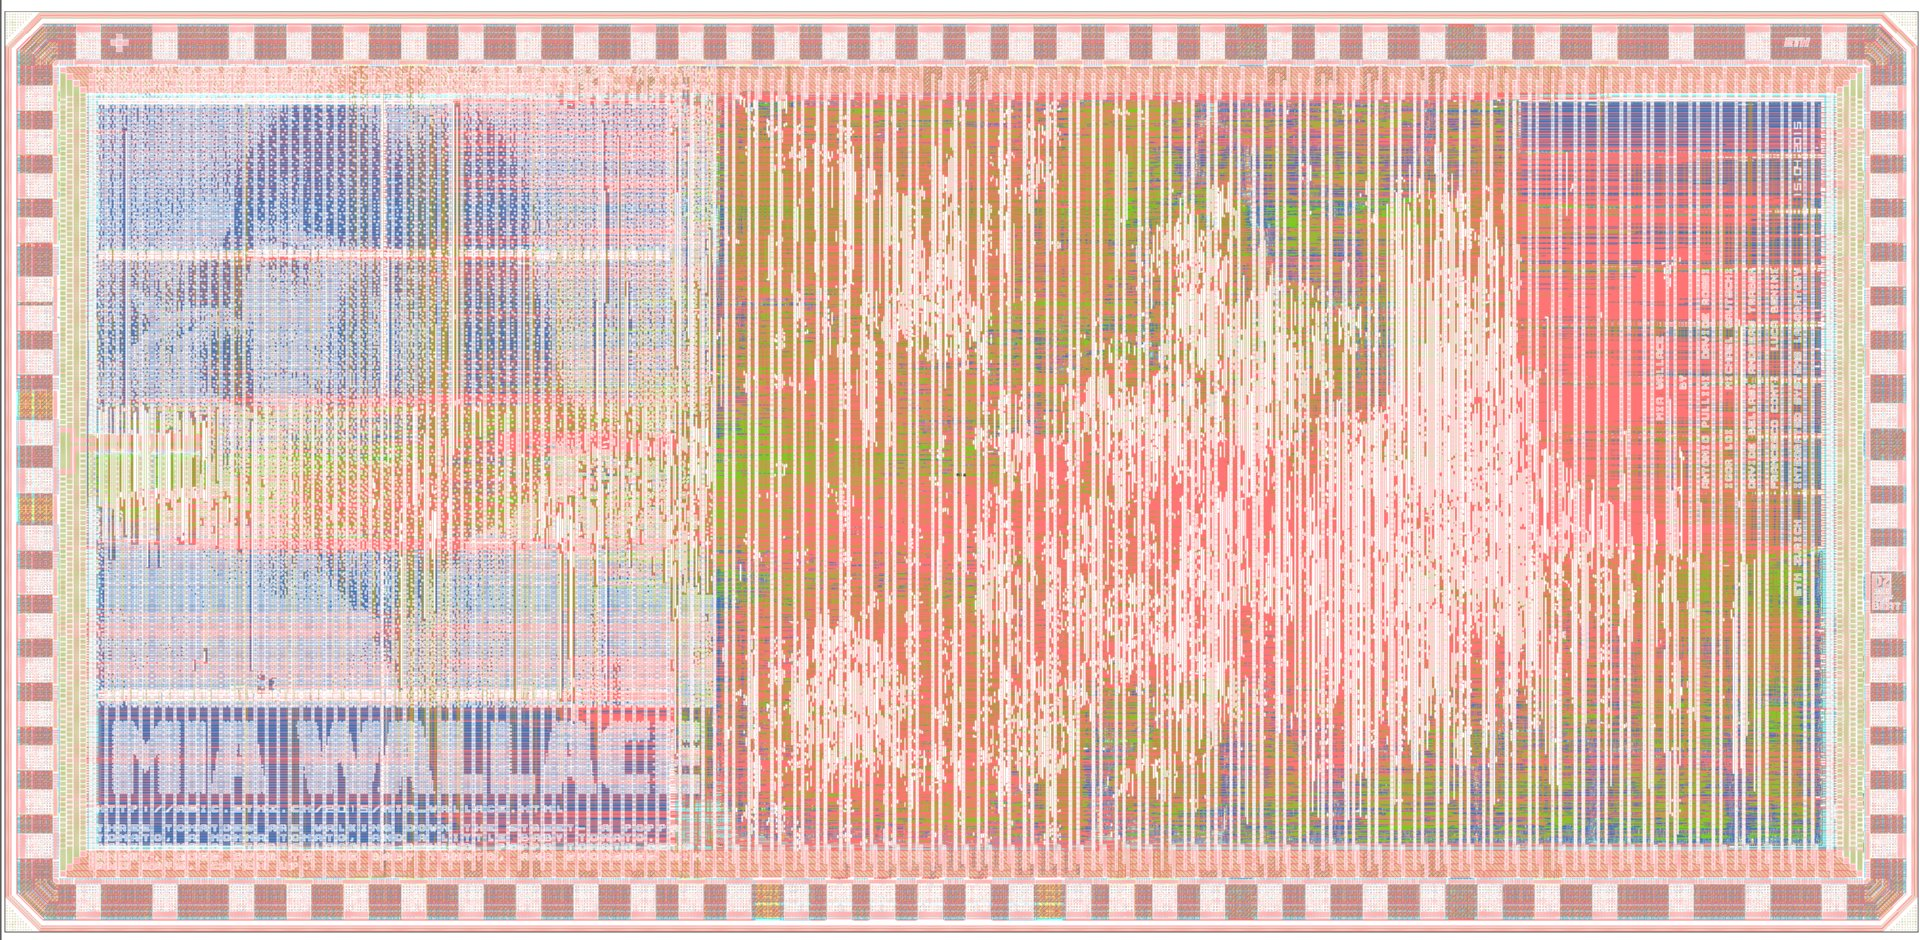
\includegraphics[width=0.9\textwidth]{./figures/mia_wallace_layout_rev_sml}
  \caption{Mia Wallace final layout.}
  \label{fig:mia_final_layout}
\end{figure}

Mia Wallace is one of the chips that were developed in the \gls{PULP}
environment. It uses one full cluster of four cores with 256 kB of L2 \gls{RAM},
64 kB of SRAM TCDM and 8 kB of SCM TCDM. Mia Wallace was designed for the 65
nm technology from UMC and tries to showcase the features of the PULP system.
Since 65 nm rather than the 28 nm FDSOI technology of pulp2 was used, we cannot
expect the same energy efficiency, instead our focus lay on the evolution of the
platform. For example we changed the processing core from the previous
chip to \orion, the core that was improved in this master thesis. A picture of
the final layout of Mia Wallace is shown in Figure~\ref{fig:mia_final_layout}.

The results presented in this chapter were all generated in the context of the
Mia Wallace chip.
This chapter is structured as follows. In Section~\ref{sec:res_performance} the
number of cycles for a set of benchmarks are compared between the OR1200 core
and \orion with different instruction set extensions enabled. Where available
also numbers for an ARM Cortex M4 are shown which allow direct comparison with
the a commercial core for embedded applications.
Section~\ref{sec:res_area} contains area and timing results for the modified
\orion core, while Section~\ref{sec:res_energy} shows the energy reduction that
can be achieved with the extended \gls{ISA}.

Note that the results related to hardware, i.e. area, timing and energy, might change
when moving to another technology. The performance figures presented here will
stay the same though.


%Among other things the instruction cache and many peripherals were heavily
%improved or rewritten from scratch compared to pulp2. We were able to improve
%the peformance by more than a factor of five compared to pulp2 while at the
%same time increase clock frequency.

% Many new feature were introduced with Mia Wallace, for example basic debugging
% support was added. With Mia it is possible to attach a debugger, for example
% gdb, via jtag to the final ASIC. The features that are supported include
% reading and writing to general-purpose registers, special-purpose registers,
% on-chip memory and using breakpoints to halt execution of the cores.


\section{Performance}

\label{sec:res_performance}

\subsection{Vectorial Instructions \& MAC Improvements}

Figure~\ref{fig:vec_cpu_comp} and Table~\ref{tab:vec_cpu_comp} show a
comparison between different evolutionary steps of the \orion OpenRISC core.
%, when
%considering vectorial instructions, misaligned accesses, hardware loops and
%pre-/post-increment load and stores.
We compare the optimized OR1200 core that was used in pulp2 and the current
state of \orion that was used in Mia Wallace. Additionally we present some
numbers for an ARM Cortex M4.

On the left hand side of this figure general purpose applications are shown
which do not perform many computations on 8 or 16 bit data types, but use mostly
32 bit data. On the right hand side we have two types of applications, first a
\gls{FIR} filter on 16 bits and three types of matrix multiplications. The first
matrix multiplication, mm8, uses 8 bit, the second, mm16, 16 bit and the third
one 32 bit integers.

Seven different \gls{CPU} profiles are shown in the figures, the first two are
performed using the GCC compiler for OpenRISC, once we used the old OR1200
\gls{CPU} and once our modified \orion core. Since this version of GCC does not
know about our extensions, it is not able to use them in any way. So both
OpenRISC \glspl{CPU} are executing exactly the same binary.
The next four profiles belong to the LLVM compiler on our modified \orion core
with different extension sets enabled.
The last profile is a Cortex M4 which uses a completely different instruction
set than OpenRISC, specifically ARMv7-M Thumb.

When comparing \orion with the OR1200 executing the same binary, we can see that
they have almost the same performance, although the OR1200 is slightly faster.
The reason for that is that we are using a simple branch predictor for \orion to
cut the critical path to the instruction cache. This was needed to achieve a
higher clock frequency compared to the OR1200 \gls{CPU}.

Comparing LLVM and GCC for \orion without our new extensions, we can see that
LLVM seems to be performing faster than GCC in almost all cases, so it seems to
be a good idea to go with the new LLVM compiler in any case. As soon as we start
enabling our \gls{ISA} extensions, we can gain a lot of performance compared to
the baseline (\orion with LLVM).

Especially on the matrix multiplication and fir benchmarks, the new MAC and
vectorial extensions achieve a speedup of up to 5x. Enabling vectorial
extensions on the matrix multiplication on 32 bit does not gain any performance
which is not surprising since there is no sub-word parallelism that the
vectorial unit could exploit. Still the new MAC extension is able to increase
the performance in this benchmark by $22\%$.



Note that no code changes were necessary to make use of the \gls{ISA}
extensions, but the new instructions were inferred automatically by our LLVM
compiler.


\begin{figure}[htbp]
  \centering
  {\scriptsize
\ref{perflegend}
}

\begin{tikzpicture}[font=\scriptsize, tight background]
\begin{axis}[
  ylabel={Speedup},
  width=.56\linewidth,
  height=.50\linewidth,
  xtick=data,
  ybar=0,
  bar width=4,
  grid,
  ymin=0.4,
  ymax=1.43,
	ytick={0.4,0.5,0.6,0.7,0.8,0.9,1,1.1,1.2,1.3,1.4},
  yticklabel style={/pgf/number format/.cd,fixed,precision=2},
  every axis y label/.style={at={(ticklabel cs:.5,5)},rotate=90},
	xticklabels={aes-cbc,sha,conv2d,fft,ipm},
	cycle list name=mylist,
  enlarge x limits=0.2,
  legend to name=perflegend,
	legend style={
		draw=none,
		legend columns=2,
		/tikz/every even column/.append style={column sep=.5cm},
    transpose legend,
    legend cell align=left
	}
  ]

	\coordinate (A) at (axis cs:0,1);
	\coordinate (O1) at (rel axis cs:0,0);
	\coordinate (O2) at (rel axis cs:1,0);
	\draw [black,sharp plot,line width=1pt] (A -| O1) -- (A -| O2);
	\pgfplotsset{cycle list shift=6};
	\addplot table [x expr=\coordindex, y expr={\thisrow{cfg}/\thisrow{cfgor1200}},col sep=comma] {data/perf-lo.csv};
	\addplot table [x expr=\coordindex, y expr={\thisrow{cfg}/\thisrow{cfgGCC}},col sep=comma] {data/perf-lo.csv};
	\pgfplotsset{cycle list shift=-2};
	\addplot table [x expr=\coordindex, y expr={\thisrow{cfg}/\thisrow{cfg}},col sep=comma] {data/perf-lo.csv};
	\addplot table [x expr=\coordindex, y expr={\thisrow{cfg}/\thisrow{cfgIH}},col sep=comma] {data/perf-lo.csv};
	\addplot table [x expr=\coordindex, y expr={\thisrow{cfg}/\thisrow{cfgIHM}},col sep=comma] {data/perf-lo.csv};
	\addplot table [x expr=\coordindex, y expr={\thisrow{cfg}/\thisrow{cfgIHVM}},col sep=comma] {data/perf-lo.csv};
	\addplot table [x expr=\coordindex, y expr={\thisrow{cfg}/\thisrow{cortexM4}},col sep=comma] {data/perf-lo.csv};
	\legend{{GCC: OR1200},{GCC: OR10N},{LLVM: OR10N},{+HWLP,LD/ST},{+HWLP,LD/ST,MAC},{+HWLP,LD/ST,MAC,VEC}, {Cortex M4}};

\end{axis}
\end{tikzpicture}
%
\begin{tikzpicture}[font=\scriptsize, tight background]
\begin{axis}[
  ylabel={Speedup},
  width=.47\linewidth,
  height=.50\linewidth,
  xtick=data,
  ybar=0,
  bar width=4,
  grid,
  ymin=0.5,
  ymax=5.2,
	ytick={0,0.5,1,1.5,2,2.5,3,3.5,4,4.5,5},
  yticklabel style={/pgf/number format/.cd,fixed,precision=2},
  every axis y label/.style={at={(ticklabel cs:.5,5)},rotate=90},
	xticklabels={fir,mm8,mm16,mm32},
  %x tick label style={rotate=0,anchor=east},
	cycle list name=mylist,
  enlarge x limits=0.2,
  ]

	\coordinate (A) at (axis cs:0,1);
	\coordinate (O1) at (rel axis cs:0,0);
	\coordinate (O2) at (rel axis cs:1,0);
	\draw [black,sharp plot,line width=1pt] (A -| O1) -- (A -| O2);
	\pgfplotsset{cycle list shift=6};
	\addplot table [x expr=\coordindex, y expr={\thisrow{cfg}/\thisrow{cfgor1200}},col sep=comma] {data/perf-hi.csv};
	\addplot table [x expr=\coordindex, y expr={\thisrow{cfg}/\thisrow{cfgGCC}},col sep=comma] {data/perf-hi.csv};
	\pgfplotsset{cycle list shift=-2};
	\addplot table [x expr=\coordindex, y expr={\thisrow{cfg}/\thisrow{cfg}},col sep=comma] {data/perf-hi.csv};
	\addplot table [x expr=\coordindex, y expr={\thisrow{cfg}/\thisrow{cfgIH}},col sep=comma] {data/perf-hi.csv};
	\addplot table [x expr=\coordindex, y expr={\thisrow{cfg}/\thisrow{cfgIHM}},col sep=comma] {data/perf-hi.csv};
	\addplot table [x expr=\coordindex, y expr={\thisrow{cfg}/\thisrow{cfgIHVM}},col sep=comma] {data/perf-hi.csv};
	\addplot table [x expr=\coordindex, y expr={\thisrow{cfg}/\thisrow{cortexM4}},col sep=comma] {data/perf-hi.csv};


\end{axis}
\end{tikzpicture}
\vspace*{-1.2em}

  \caption{Vectorial instruction speedup.}
  \label{fig:vec_cpu_comp}
\end{figure}

\begin{table}[H]
 \caption{Vectorial instructions: number of cycles.}
 \label{tab:vec_cpu_comp}
% \hspace*{-40pt}
 \begin{threeparttable}
 \begin{tabular}{@{}l|r|r|r|r|r|r@{}} \toprule
  \textbf{Features}    & OR1200      & \orion     &      \orion & \orion                        & \orion  & ARM Cortex M4\tnote{3} \   \\
                       & GCC         & GCC        &        LLVM & LLVM\tnote{1} \, & LLVM\tnote{1,2} \,\, & GCC\\ \midrule
  \textbf{aes\_cbc}    &      49126  &      49819 &       40607 &      35383 &  34339  &  42202 \\
  \textbf{sha}         &      49615  &      49665 &       50191 &      40853 &  37414  &  43437 \\
  \textbf{conv2d}      &       5936  &       5943 &        5211 &       4581 &   3696  &   5453 \\
  \textbf{fft}         &      49800  &      50583 &       43068 &      42093 &  41193  &  57960 \\
  \textbf{ipm}         &       4579  &       4701 &        2552 &       2407 &   2407  &   3103 \\
  \textbf{fir}         &      24937  &      25128 &       19437 &      11463 &   9468  &  19122 \\
  \textbf{mm8}         &     376444  &     377534 &      315216 &     173537 &  62209  & 280225 \\
  \textbf{mm16}        &     377889  &     378531 &      316260 &     175687 &  90006  & 280477 \\
  \textbf{mm32}        &     311937  &     312995 &      316254 &     179037 & 146269  & 247548 \\
  \bottomrule
 \end{tabular}
 \begin{tablenotes}
  \item [1] Hardware loops, pre-/post-increment load and stores
  \item [2] Vectorial instructions, new MAC, misaligned access
  \item [3] An STM32F429ZI \cite{STM32F429} MCU by STMicroeletronics was used
 \end{tablenotes}
 \end{threeparttable}
\end{table}

\clearpage

\subsection{Bit Counting Instructions}

Bit counting instructions are only seldom used, but if they can be inferred,
they show a massive speedup as shown in Figure~\ref{fig:bit_count_cpu_comp}. The
bitDescriptor benchmark uses the \instr{l.ff1} instruction to find bits that are set
in a word and performs an action based on the index of those bits. The second
benchmark, KP Matching, performs image key point matching and heavily uses the
\instr{l.cnt} instruction to calculate hamming weights.

\begin{figure}[htbp]
  \centering
  {\scriptsize
\ref{perflegend2}
}

\hspace{5em}
\begin{tikzpicture}[font=\scriptsize, tight background]
\begin{axis}[
  ylabel={Speedup},
  width=.30\linewidth,
  height=7.5cm,
  xtick=data,
  ybar=0,
  bar width=6.5,
  grid,
  ymin=0.6,
  ymax=3.8,
	ytick={0.6,1,1.4,1.8,2.2,2.6,3.0,3.4,3.8},
  yticklabel style={/pgf/number format/.cd,fixed,precision=2},
  every axis y label/.style={at={(ticklabel cs:.5,5)},rotate=90},
	xticklabels={bitDesc.},
	cycle list name=mylist,
  enlarge x limits=0.4,
  legend to name=perflegend2,
	legend style={
		draw=none,
		legend columns=2,
		/tikz/every even column/.append style={column sep=.5cm},
    transpose legend,
    legend cell align=left
	}
  ]

	\coordinate (A) at (axis cs:0,1);
	\coordinate (O1) at (rel axis cs:0,0);
	\coordinate (O2) at (rel axis cs:1,0);
	\draw [black,sharp plot,line width=1pt] (A -| O1) -- (A -| O2);
	\addplot table [x expr=\coordindex, y expr={\thisrow{cfg}/\thisrow{cfg}},col sep=comma] {data/perf-bit.csv};
	\addplot table [x expr=\coordindex, y expr={\thisrow{cfg}/\thisrow{cfgIH}},col sep=comma] {data/perf-bit.csv};
	\pgfplotsset{cycle list shift=1};
	\addplot table [x expr=\coordindex, y expr={\thisrow{cfg}/\thisrow{cfgIHVM}},col sep=comma] {data/perf-bit.csv};
	\pgfplotsset{cycle list shift=2};
	\addplot table [x expr=\coordindex, y expr={\thisrow{cfg}/\thisrow{cfgIHVMC}},col sep=comma] {data/perf-bit.csv};
	\legend{Base,{+HWLP,LD/ST},{+HWLP,LD/ST,MAC,VEC},{+HWLP,LD/ST,MAC,VEC,BIT}};
\end{axis}
\end{tikzpicture}
\hspace{1em}
\begin{minipage}[c][0cm]{0.45\linewidth}
\vspace{45pt}
\begin{tikzpicture}[font=\scriptsize, tight background]
\begin{groupplot}[
    group style={
        group name=my fancy plots,
        group size=1 by 2,
        xticklabels at=edge bottom,
        vertical sep=0pt
    },
  width=0.7\linewidth,
  xtick=data,
  ybar=0,
  grid,
  every axis y label/.style={at={(ticklabel cs:.5,5)},rotate=90},
	xticklabels={KP Matching},
	cycle list name=mylist,
  enlarge x limits=0.4,
]
%
\nextgroupplot[ymin=30,ymax=36,
               ytick={34,35,36},
               axis x line=none, 
               axis y discontinuity=crunch,
               height=4.1cm]
	\coordinate (A) at (axis cs:0,1);
	\coordinate (O1) at (rel axis cs:0,0);
	\coordinate (O2) at (rel axis cs:1,0);
	\addplot table [x expr=\coordindex, y expr={\thisrow{cfg}/\thisrow{cfg}},col sep=comma] {data/perf-bit2.csv};
	\addplot table [x expr=\coordindex, y expr={\thisrow{cfg}/\thisrow{cfgIH}},col sep=comma] {data/perf-bit2.csv};
	\pgfplotsset{cycle list shift=1};
	\addplot table [x expr=\coordindex, y expr={\thisrow{cfg}/\thisrow{cfgIHVM}},col sep=comma] {data/perf-bit2.csv};
	\pgfplotsset{cycle list shift=2};
	\addplot table [x expr=\coordindex, y expr={\thisrow{cfg}/\thisrow{cfgIHVMC}},col sep=comma] {data/perf-bit2.csv};
%
\nextgroupplot[ymin=0,ymax=1.5,
               ytick={0,0.2,0.4,0.6,0.8,1,1.2},
               axis x line=bottom,
               height=5.0cm]
	\coordinate (A) at (axis cs:0,1);
	\coordinate (O1) at (rel axis cs:0,0);
	\coordinate (O2) at (rel axis cs:1,0);
	\draw [black,sharp plot,line width=1pt] (A -| O1) -- (A -| O2);
	\addplot table [x expr=\coordindex, y expr={\thisrow{cfg}/\thisrow{cfg}},col sep=comma] {data/perf-bit2.csv};
	\addplot table [x expr=\coordindex, y expr={\thisrow{cfg}/\thisrow{cfgIH}},col sep=comma] {data/perf-bit2.csv};
	\pgfplotsset{cycle list shift=1};
	\addplot table [x expr=\coordindex, y expr={\thisrow{cfg}/\thisrow{cfgIHVM}},col sep=comma] {data/perf-bit2.csv};
	\pgfplotsset{cycle list shift=2};
	\addplot table [x expr=\coordindex, y expr={\thisrow{cfg}/\thisrow{cfgIHVMC}},col sep=comma] {data/perf-bit2.csv};

  ylabel={Speedup},
	xticklabels={KP Matching},
	cycle list name=mylist,
\end{groupplot}
\end{tikzpicture}
\end{minipage}

  \caption{Bit counting instructions.}
  \label{fig:bit_count_cpu_comp}
\end{figure}

Our other extensions only give us a speedup of 32\% and 11\% respectively and
the new MAC and vectorial instructions do not give us any additional speedup at
all, while the bit counting extension gives us a speedup of 3.6x and 35x
respectively.



\section{Area \& Timing}
\label{sec:res_area}

Figure~\ref{fig:area_inc} shows the area impact of our new extensions in the
core and cluster. Those numbers were calculated by using the final Mia Wallace
setup, selectively removing our instruction set extensions and performing
synthesis runs.
The area of the OpenRISC core was increased by $25\%$ in total from 35.5 kGE to
44.5 kGE when considering all extensions. When we only consider vectorial
instructions, bit counting and the improved MAC unit, the increase of core area
diminishes to only $10\%$.
If we look at the cluster area, the area impact is even less visible and
consists of about $2\%$ for all extensions together.
Comparing those numbers with the OR1200 CPU which needed an area of 37.9 kGE, we
see that \orion is a little bit smaller than the OR1200 when we are not using
any of our extensions. By adding all extensions, the area of \orion increases,
so in the end our final \orion core is $17\%$ larger than the OR1200, but has a
much higher execution speed.

\begin{figure}[H]
  \centering
  \ref{areapowerlegend}

\hspace*{-1em}
\begin{tikzpicture}[font=\scriptsize, tight background]
\begin{axis}[
  ylabel={Area [$kGE$]},
  width=.65\linewidth,
  height=1.1\linewidth,
  ybar=0pt,
	xtick=data,
  bar width=5,
  ymin=0,
  grid,
  yticklabel style={font=\tiny,/pgf/number format/.cd,fixed,precision=1},
  every axis y label/.style={at={(ticklabel cs:.5,5)},rotate=90},
	xticklabels={Core},
	cycle list name=mylist,
  enlarge x limits=0.3,
	legend to name=areapowerlegend,
	legend style={
		draw=none,
		legend columns=1,
		/tikz/every even column/.append style={column sep=.5cm},
    transpose legend,
    legend cell align=left
  },
  ]

\addplot table [x expr=\coordindex, y=base,col sep=comma] {data/area.csv};
\addplot table [x expr=\coordindex, y=cfgIH,col sep=comma] {data/area.csv};
\addplot table [x expr=\coordindex, y=cfgIHM,col sep=comma] {data/area.csv};
\addplot table [x expr=\coordindex, y=cfgIHVM,col sep=comma] {data/area.csv};
\pgfplotsset{cycle list shift=1};
\addplot table [x expr=\coordindex, y=cfgIHVMC,col sep=comma] {data/area.csv};
%	\legend{Base,{+HWLP,LD/ST},{+HWLP,LD/ST,MAC},{+HWLP,LD/ST,MAC,VEC}};

\end{axis}
\end{tikzpicture}
\begin{tikzpicture}[font=\scriptsize, tight background]
\begin{axis}[
	ylabel near ticks,
	yticklabel pos=right,
  width=.65\linewidth,
  height=1.1\linewidth,
  ybar=0pt,
  ymin=1400,
	xtick=data,
  bar width=5,
  ymin=0,
  grid,
  yticklabel style={font=\tiny,/pgf/number format/.cd,fixed,precision=1},
  every axis y label/.style={at={(ticklabel cs:.5,5)},rotate=90},
	xticklabels={Cluster},
	cycle list name=mylist,
  enlarge x limits=0.3,
  ]

\addplot table [x expr=\coordindex, y=base,col sep=comma] {data/area-cluster.csv};
\addplot table [x expr=\coordindex, y=cfgIH,col sep=comma] {data/area-cluster.csv};
\addplot table [x expr=\coordindex, y=cfgIHM,col sep=comma] {data/area-cluster.csv};
\addplot table [x expr=\coordindex, y=cfgIHVM,col sep=comma] {data/area-cluster.csv};
\pgfplotsset{cycle list shift=1};
\addplot table [x expr=\coordindex, y=cfgIHVMC,col sep=comma] {data/area-cluster.csv};

\end{axis}
\end{tikzpicture}

  \caption{Area overhead.}
  \label{fig:area_inc}
\end{figure}

\begin{table}[H]
 \caption{Area overhead}
 \label{tab:area_inc}
 \centering\begin{tabular}{@{}lrr@{}} \toprule
   \textbf{Feature}  & \textbf{Area}    & \\ \toprule
   \drawbar{gray!20}   Baseline         & 35.5 kGE &         \\ \hline
   \drawbar{blue!60}   HWLP             &  3.0 kGE &  +8.5\%   \\ \hline
   \drawbar{blue!60}   Reg. File Add.   &  3.7 kGE & +10.4\%   \\ \hline
   \drawbar{red!60}    New MAC          &  1.2 kGE &  +3.3\%   \\ \hline
   \drawbar{orange!60} Vectorial ALU    &  1.9 kGE &  +5.3\%   \\ \hline
   \drawbar{green!60}  Bit Count        &  0.2 kGE &  +0.8\%   \\ \midrule
                       \textit{Total}   & \textit{44.5 kGE} &  \\ \bottomrule
  \end{tabular}
\end{table}

All our new instruction set extensions did not increase the critical path of the
\orion. In the slow corner of the UMC 65 technology with $1.08$ V supply
voltage, we achieved a clock period of $2.23$ ns for \orion and a clock period
of $2.4$ ns for OR1200 after synthesis, meaning that also in terms of frequency
our new core is faster than the original one.


\section{Energy}
\label{sec:res_energy}

For some of the benchmarks mentioned above we performed a power estimation on
the final Mia Wallace netlist, see Figure~\ref{fig:vectorial_energy} for the
results. It can be seen that we did not only achieve a higher performance compared to
original OpenRISC ISA, but also need less energy. This is not surprising as can
be seen when we compare the average power used by the core and cluster. It is
true that more power is used when our extensions are active, but the
applications run much faster and thus the core needs to stay active for a
shorter amount of time.


\begin{figure}[htbp]
  \centering
  \ref{energylegend}

\begin{tikzpicture}[font=\scriptsize, tight background]
\begin{axis}[
  ylabel={Normalized Core Energy},
  width=0.55\linewidth,
  height=.5\linewidth,
  ybar=0pt,
	xtick=data,
  bar width=5,
  grid,
  ymin=0.2,
  ymax=1.3,
  ytick={0.2,0.4,0.6,0.8,1,1.2},
  yticklabel style={font=\tiny,/pgf/number format/.cd,fixed,precision=1},
  every axis y label/.style={at={(ticklabel cs:.5,5)},rotate=90},
	xticklabels={mm8, mm16, mm32, fir, fft},
	cycle list name=mylist,
  enlarge x limits=0.2,
	legend to name=energylegend,
	legend style={
		draw=none,
		legend columns=1,
		/tikz/every even column/.append style={column sep=.5cm},
    transpose legend,
    legend cell align=left
  },
  ]

	\coordinate (A) at (axis cs:0,1);
	\coordinate (O1) at (rel axis cs:0,0);
	\coordinate (O2) at (rel axis cs:1,0);
	\draw [black,sharp plot,line width=1pt] (A -| O1) -- (A -| O2);
	\addplot table [x expr=\coordindex, y=base,col sep=comma] {data/energy.csv};
	\pgfplotsset{cycle list shift=1};
	\addplot table [x expr=\coordindex, y=cfgIHM,col sep=comma] {data/energy.csv};
	\addplot table [x expr=\coordindex, y=cfgIHVM,col sep=comma] {data/energy.csv};
	%\addplot table [x expr=\coordindex, y=cortexM4,col sep=comma] {data/energy.csv};
	\legend{Base,{+HWLP,LD/ST,MAC},{+HWLP,LD/ST,MAC,VEC}};

\end{axis}
\end{tikzpicture}
\hspace{2em}
\begin{tikzpicture}[font=\scriptsize, tight background]
\begin{axis}[
  ylabel={Avg. Power [$mW$]},
  width=.25\linewidth,
  height=.5\linewidth,
  xtick=data,
  ybar=0pt,
  ymin=0,
  bar width=5,
  grid,
  yticklabel style={font=\tiny,/pgf/number format/.cd,fixed,precision=1},
  every axis y label/.style={at={(ticklabel cs:.5,5)},rotate=90},
	xticklabels={Core,1-core cluster, 4-core cluster},
  enlarge x limits=0.2,
	cycle list name=mylist,
  ]

\addplot table [x expr=\coordindex, y=base,col sep=comma] {data/power.csv};
\pgfplotsset{cycle list shift=1};
\addplot table [x expr=\coordindex, y=cfgIHM,col sep=comma] {data/power.csv};
\addplot table [x expr=\coordindex, y=cfgIHVM,col sep=comma] {data/power.csv};

\end{axis}
\end{tikzpicture}
\begin{tikzpicture}[font=\scriptsize, tight background]
\begin{axis}[
	ylabel near ticks,
	yticklabel pos=right,
  width=.25\linewidth,
  height=.5\linewidth,
  xtick=data,
  ybar=0pt,
  ymin=0,
  bar width=5,
  grid,
  yticklabel style={font=\tiny,/pgf/number format/.cd,fixed,precision=1},
  every axis y label/.style={at={(ticklabel cs:.5,5)},rotate=90},
	xticklabels={Cluster},
  enlarge x limits=0.2,
	cycle list name=mylist,
  ]

\addplot table [x expr=\coordindex, y=base,col sep=comma] {data/power-cluster.csv};
\pgfplotsset{cycle list shift=1};
\addplot table [x expr=\coordindex, y=cfgIHM,col sep=comma] {data/power-cluster.csv};
\addplot table [x expr=\coordindex, y=cfgIHVM,col sep=comma] {data/power-cluster.csv};

\end{axis}
\end{tikzpicture}
\vspace*{-0.9em}

  \caption{Energy efficiency compared to base \gls{ISA}.}
  \label{fig:vectorial_energy}
\end{figure}

